% Chapter Template

\chapter{Behavioral Frameworks} % Main chapter title

\label{Chapter5} % Change X to a consecutive number; for referencing this chapter elsewhere, use \ref{ChapterX}

\lhead{Chapter 5. \emph{Behavioral Frameworks}} % Change X to a consecutive number; this is for the header on each page - perhaps a shortened title

\section{Requirements}
The users of social robots do not have necessary backgrounds in programming and design of robot behaviors. This lead to the development of several visual programming languages which allow non-programmers to create robot applications. Most of the available visual programming softwares allows to choose among many prebuilt behavioral blocks and connecting them to one another to get the desired flow of action \cite{MSRS4},\cite{Choregraphe}. These programs are very intuitive and allow the users to realize complex sequence of movements and sequential behaviors. But programming dynamic behaviors still remains challenging. This is primarily due to fact that the users have to think about the data flow between various blocks by appropriate connections between them. When it comes to designing complex dynamic behaviors this task becomes very tedious and time consuming. 
Programming complex dynamic behaviors for small commercial humanoid robots is a complicated task for the inexperienced roboticists\cite{BerenzTDM2014} for the following reasons.
\begin{itemize}
\item Synchronizing the data flow between tasks that run at different rates
\item Ensuring robustness and task continuity in case of unreliable sensory modules
\item Providing memory infrastructure to manage the existence and positions of detected objects
\item Organizing the distinct information flow for each detected object from sensory modules to processing modules
\item Conditional selection of actions and retrying in case of failure. 
\end{itemize}
\section{Existing Solutions}
There are many solutions  proposed in the literature that address the dynamic control problem. For instance Gostai's Universal Robotic Body Interface(URBI)\cite{Baillie4814281} and Task description language (TDL)\cite{Simmons724883} are programming languages developed specifically for robot programming. URBI provides a modern object-oriented scripting language that allows the organization of code into different processes that either run sequentially or in parallel, and it also provides tools for process execution monitoring. In TDL which was developed as a C++ extension, the code is organized into task trees, which encode the hierarchical decomposition of tasks as well as the synchronization of constraints between tasks.
%Apart from these, a large range of robotic architectures have been proposed, including solutions based on hierarchical control architectures \cite{Firby:1989:AEC:916113}, reactive architectures \citep{Brooks:1991:RLC:106552.106553}, and hybrid systems \citep{arkinetal},\cite{Bonasso},\cite{berra}. 
More recently, specialized operating systems have been proposed, such as ROS\cite{quigley2009ros}, which organize code into distributed asynchronous modules that exchange data using a data subscription protocol. Hierarchical organization of behaviors and modularity are also being investigated \cite{Jaegeretal},\cite{Baldassarre:2013:CRM:2560111},\cite{hurdus4648045}. These solutions manage the integration and communication between different types of hardware and software and support the implementation of reaction, as well as behavioral specification. However, these programs have been produced by robot developers and are targeted at this community, which means that they are not intended to be used by non-roboticists and a solid background in computer science/robotics is required for their use.
\begin{figure}[H]
\centering
\begin{subfigure}[b]{0.5\textwidth}
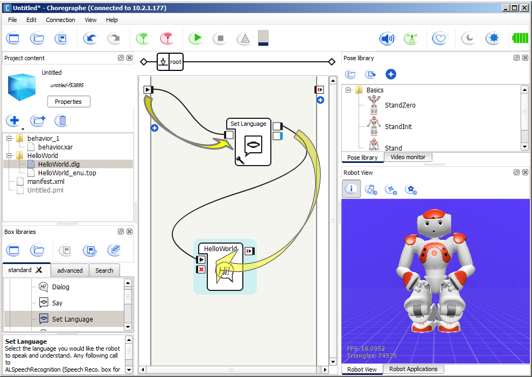
\includegraphics[width=\textwidth]{assets/helloworld_cho_dlg_05.png}
%http://doc.aldebaran.com/2-1/getting_started/helloworld_choregraphe_dialog.html
\caption{Choreographe Albebaran}
\label{fig:choreographe}
\end{subfigure}%
\begin{subfigure}[b]{0.5\textwidth}
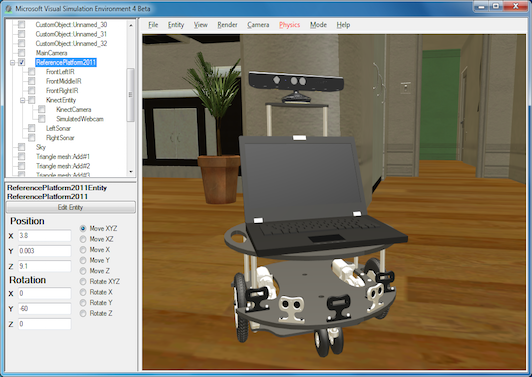
\includegraphics[width=\textwidth]{assets/MSRD4_VSE2.png}
%http://www.microsoftstore.com/store/msusa/en_US/pdp/Kinect-for-Windows-v2-Sensor/productID.298810500
\caption{MSRD Studio 4:Visual Simulation Environment}
\label{fig:msrd4_vse}
\end{subfigure}%
\caption[Visual Programming Tools]{Visual Programming Tools. {Adapted from manufacturer's site}}
\label{fig:visprog}
\end{figure}
\section{Target Drives Means Framework}
A new non-domain-specific solution called \emph{Target Drives Means (TDM)}( Developed at University of Tsukuba, Artificial Intelligence Laboratory) is proposed in \cite{BerenzTDM2014} taking into account the following requirements. 
\begin{itemize}
\item Full support for dynamic actions $\rightarrow$ Management of automatic information flow between sensory and action components, object permanence, action continuity.
\item Declarative approach and not of flowcharts, which lead to plan composition issues. 
\item Ability to specify context-specific activation of actions. 
\item Shorter learning curve. 
\item Modular design to ensure the efficient reuse
of components.
\end{itemize}
%In order to satisfy the aforementioned requirements, TDM proposes a programming paradigm where actions are not organized in a temporal sequence. Programming is achieved by specifying a collection of behaviors that run in parallel. The proposed approach allows users to design dynamic behaviors by selecting preprogrammed components from an a priori known list and associating them. The logic of the program is not expressed using communication links in a flowchart, but by the use of specialized dynamic components that regulate the activation status and the priorities of the behaviors. 
%
%Users can apply TDM to create programs by associating preprogrammed components from an organized library as shown in Figure~\ref{fig:tdm_comp}. There are four types of components:
%\begin{itemize}
%\item \emph{Functions} for actions or the handling of sensory data.
%\item \emph{Conditions} that monitor the activation status of functions.
%\item \emph{Score calculators} that perform the online evaluation of the execution priority for clusters of functions known as behaviors.
%\item \emph{Triggers} that link sensing to acting.
%\end{itemize}
%
%The functions, conditions and score calculators are all dynamic components. If the user adds one of these components to a program, the architecture connects it automatically to a central memory called the Internal Model (IM). The components never communicate with each other directly because information exchange occurs via the IM. The IM organizes the information flow between connected components, which makes dynamic control and management of memory of objects a simple task. The priority of execution of the tasks are dynamically controlled using the result of the score calculator associated with each behavior as shown in Figure~\ref{fig:tdm_priority}.
%
%\begin{figure}[H]
%\centering
%\begin{subfigure}[b]{0.45\textwidth}
%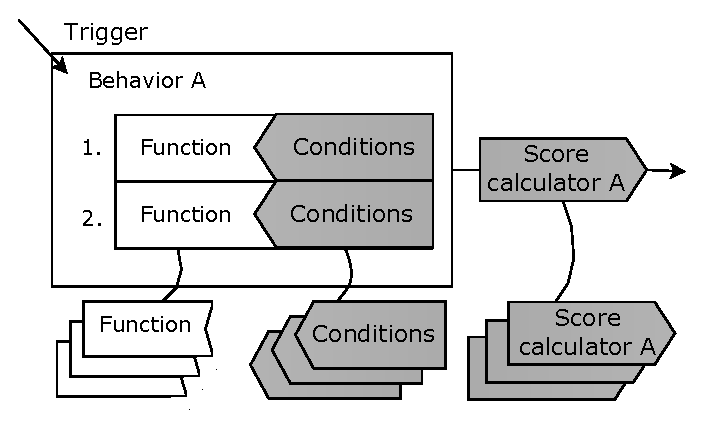
\includegraphics[width=\textwidth]{assets/tdm_components.eps}
%\caption{Behavior programming from component library}
%\label{fig:tdm_comp}
%\end{subfigure}%
%\hfill
%\begin{subfigure}[b]{0.4\textwidth}
%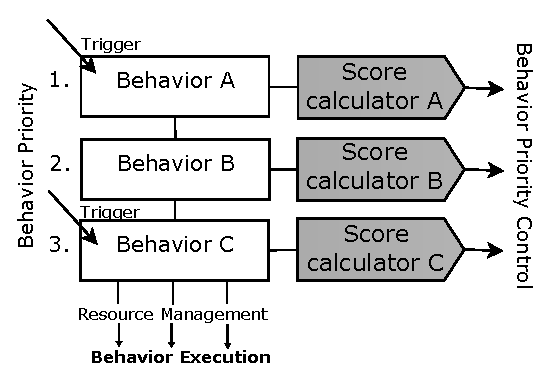
\includegraphics[width=\textwidth]{assets/tdm_priority.eps}
%\caption{Behavior coordination and execution}
%\label{fig:tdm_priority}
%\end{subfigure}%
%\caption{TDM primitives and concepts}
%\label{fig:tdm1}
%\end{figure}
%
%An example of the minimal program using TDM paradigm is shown in Figure~\ref{fig:tdm_example} for the dynamic ball kicking problem. There are two behaviors specified in the example program one of which is the default behavior. There are two functions inside the default behavior which are "Ball detection" function which pushes the position of the ball to the internal model when one is detected. There is also the "Move head left right" function which searches for the presence of the ball. Within a behavior the priority of execution of the functions are controlled by the order in which the functions are arranged in this case "Ball detection" function has higher priority to the "Move head" function. The condition of execution of the functions in default behavior is always true which means that these functions will always be executed once the behavior is activated. Additionally the execution of the default behavior doesn't need external trigger which means the default behavior will always be executed. The score calculator of the default behavior is set to 0 which means that the default behavior will be executed with low priority. Now coming to the "Behavior 1" which performs the actual task of kicking the ball contains three functions "Head Tracking", "Kicking" and "Walking" functions. This behavior will be triggered when a ball is detected. Once the ball is detected, the "Head tracking" function retrieves the position of the ball from the internal model and starts to track it. The "Walking" function instead makes sure that the robot walks towards the ball. These two functions will execute unconditionally once "Behavior 1" is activated. However once the robot comes close to the ball the condition of vicinity will be satisfied and the "Kicking" function will be activated and the robot kicks the ball. 
%
%\begin{figure}[H]
%\centering
%\begin{subfigure}[b]{0.48\textwidth}
%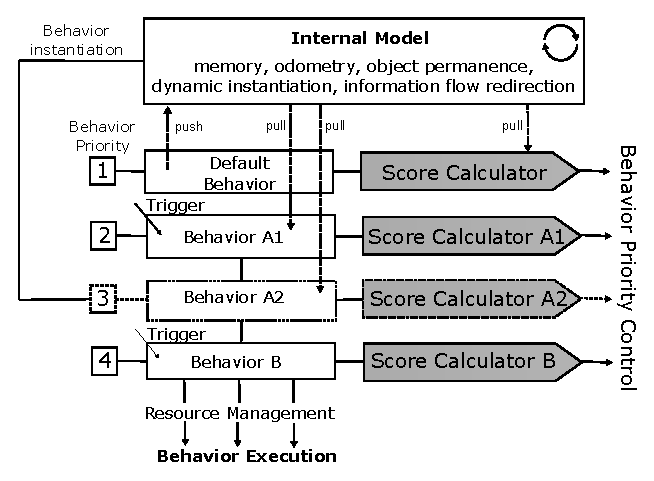
\includegraphics[width=\textwidth]{assets/tdm_im.eps}
%\caption{Information management by IM of TDM}
%\label{fig:tdm_im}
%\end{subfigure}%
%\hfill
%\begin{subfigure}[b]{0.45\textwidth}
%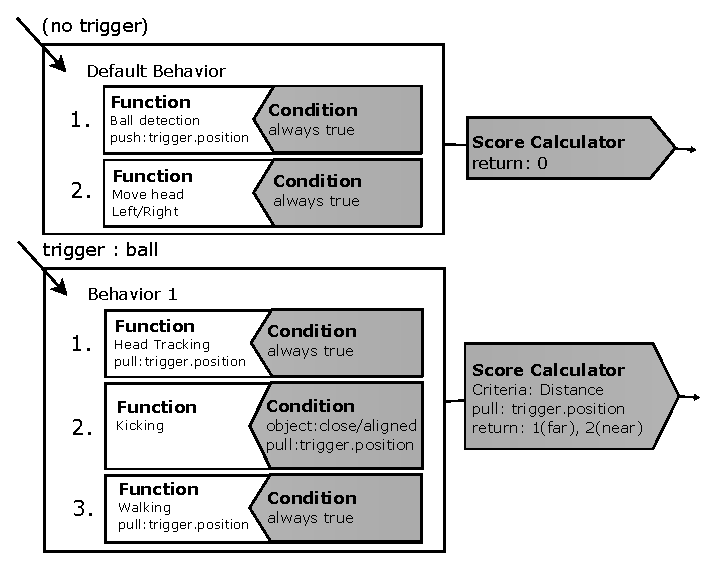
\includegraphics[width=\textwidth]{assets/tdm_example.eps}
%\caption{An example Program in TDM}
%\label{fig:tdm_example}
%\end{subfigure}%
%\caption{TDM Framework \cite{BerenzTDM2014}}
%\label{fig:tdm2}
%\end{figure}
%
%The communication between components through IM is shown in Figure~\ref{fig:tdm_im}. Now let us see how the IM makes the dynamic behavior control problem easier. The IM organizes the information flows between components. It implements odometry, manages the notion of object permanence, and redirects information based on the trigger components. The IM runs its own process and uses the pull/push communication system, which allows asynchronous exchange of data. The redirection of information from sensing functions to other components is nontrivial if several objects of the same type are detected. As mentioned previously, the detection of several balls implies a risk of incoherent behavior, where the robot will switch constantly between walking toward one ball and walking toward another ball. The IM solves this issue in a transparent manner as follows.
%\begin{itemize}
%\item Behaviors are generated at run-time according to triggers, i.e., if two balls are detected, two behaviors are created during runtime.
%\item Two distinct information flows are enforced between the sensory functionality and the two dynamically created behaviors.
%\end{itemize}
%The IM achieves this by processing the information coming from sensory modules through push connections into knowledge about distinct objects, creating and maintaining a scheme representation for each object. In the case of balls:
%\begin{itemize}
%\item The IM compares all of the ball schemes pushed by the ball detection function to several dynamically created reference schemes.
%\item The IM updates the properties of these two reference schemes based on the properties of similar pushed schemes.
%\item The IM replies to pull requests from the two distinct behaviors with a suitable scheme, thereby enforcing two distinct control
%loops.
%\end{itemize}
%The maintenance of reference schemes that are used as buffers between sensing and acting solves the problems with continuity of action in the context of unreliable sensory modules.
%At the time of publication of \cite{BerenzTDM2014}, a visual programming software using TDM was not developed however the user studies were done to understand the usability of such a dynamic behavior programming paradigm. The comparison results of TDM and Aldebaran Choreographe for a number of tasks shown in Figure~\ref{fig:tdm_casestudy1} was conducted and a comparison of the programming time required for each of these tasks is shown in Figure~\ref{fig:tdm_casestudy2}. It could be noted that TDM could be effectively used for designing complex dynamic behaviors.
%
%\begin{figure}[H]
%\centering
%\begin{subfigure}[b]{0.48\textwidth}
%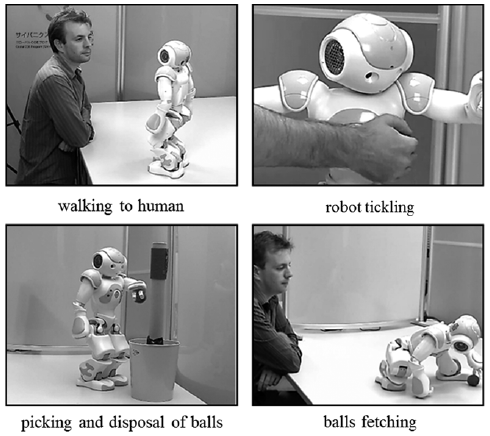
\includegraphics[width=\textwidth]{assets/tdm_casestudy1.png}
%\caption{TDM behaviors used for evaluation}
%\label{fig:tdm_casestudy1}
%\end{subfigure}%
%\hfill
%\begin{subfigure}[b]{0.45\textwidth}
%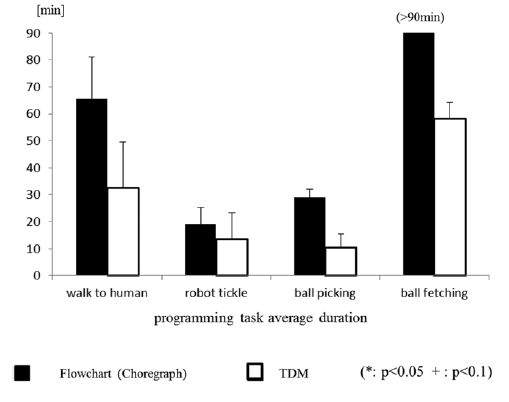
\includegraphics[width=\textwidth]{assets/tdm_casestudy2.png}
%\caption{Programming time for TDM vs Choreographe}
%\label{fig:tdm_casestudy2}
%\end{subfigure}%
%\caption{TDM Usability Study \cite{BerenzTDM2014}}
%\label{fig:tdm_casestudy}
%\end{figure}
In order to satisfy the aforementioned requirements, TDM proposes a programming paradigm where temporal independent dynamic behaviors blocks run in parallel. The logic of the program is not expressed using communication links in a flowchart, but by the use of specialized dynamic components that regulate the activation status and the priorities of the behaviors. There are four types of dynamic components: \emph{Functions} for actions or the handling of sensory data, \emph{Conditions} that monitor the activation status of functions, \emph{Score calculators} that perform the online evaluation of the execution priority of behaviors, \emph{Triggers} that link sensing to acting. The components never communicate with each other directly because information exchange occurs via a specialized centralized memory called \emph{Internal Model(IM)} which takes care of asynchronous information flow (push/pull communication) between connected components, odometry, object permanence, and activation of behaviors through triggers. Figure~\ref{fig:tdm_priority} shows how the behavior prioritization is managed while Figure~\ref{fig:tdm_im} shows the complete architecture of TDM with Internal model. The IM solves the problem of data consistency and information flow if a redundant behavior has to be performed over many objects in the environment by generating the behaviors at run-time according to the trigger. Also it establishes distinct information flow between the sensor module and the behavior module.
\begin{figure}[H]
\centering
%\begin{subfigure}[b]{0.45\textwidth}
%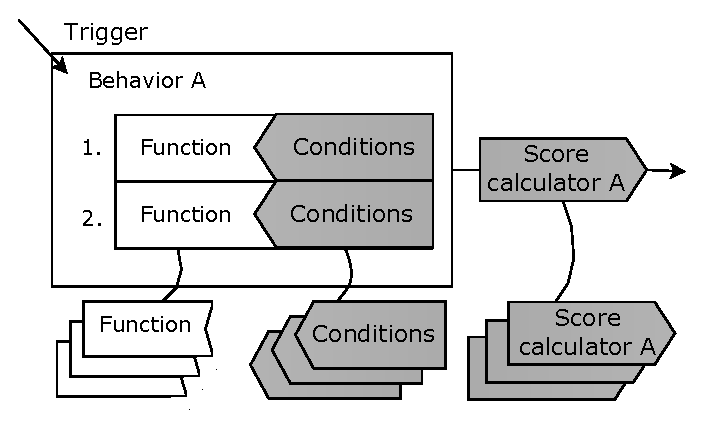
\includegraphics[width=\textwidth]{assets/tdm_components.eps}
%\caption{Behavior programming from component library}
%\label{fig:tdm_comp}
%\end{subfigure}%
%\hfill
\begin{subfigure}[b]{0.45\textwidth}
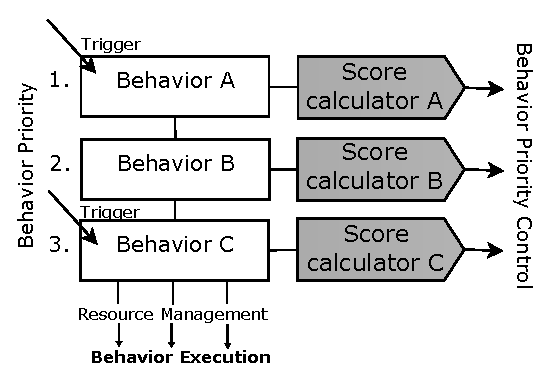
\includegraphics[width=\textwidth]{assets/tdm_priority.eps}
\caption{Behavior coordination and execution}
\label{fig:tdm_priority}
\end{subfigure}%
\hfill
\begin{subfigure}[b]{0.45\textwidth}
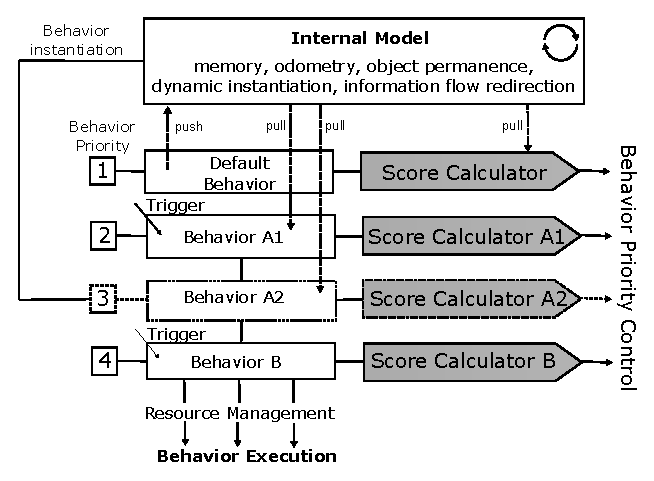
\includegraphics[width=\textwidth]{assets/tdm_im.eps}
\caption{Information management by IM of TDM}
\label{fig:tdm_im}
\end{subfigure}%
\caption[Target-drives-means Framework]{TDM Framework. {Adapted from \cite{BerenzTDM2014}}}
\label{fig:tdm1}
\end{figure}
%An example of the minimal program using TDM paradigm is shown in Figure~\ref{fig:tdm_example} for the dynamic ball kicking problem. There are two behaviors specified in the example program one of which is the default behavior. There are two functions inside the default behavior which are "Ball detection" function which pushes the position of the ball to the internal model when one is detected. There is also the "Move head left right" function which searches for the presence of the ball. Within a behavior the priority of execution of the functions are controlled by the order in which the functions are arranged in this case "Ball detection" function has higher priority to the "Move head" function. The condition of execution of the functions in default behavior is always true which means that these functions will always be executed once the behavior is activated. Additionally the execution of the default behavior doesn't need external trigger which means the default behavior will always be executed. The score calculator of the default behavior is set to 0 which means that the default behavior will be executed with low priority. Now coming to the "Behavior 1" which performs the actual task of kicking the ball contains three functions "Head Tracking", "Kicking" and "Walking" functions. This behavior will be triggered when a ball is detected. Once the ball is detected, the "Head tracking" function retrieves the position of the ball from the internal model and starts to track it. The "Walking" function instead makes sure that the robot walks towards the ball. These two functions will execute unconditionally once "Behavior 1" is activated. However once the robot comes close to the ball the condition of vicinity will be satisfied and the "Kicking" function will be activated and the robot kicks the ball. 
%
%\begin{figure}[H]
%\centering
%\begin{subfigure}[b]{0.48\textwidth}
%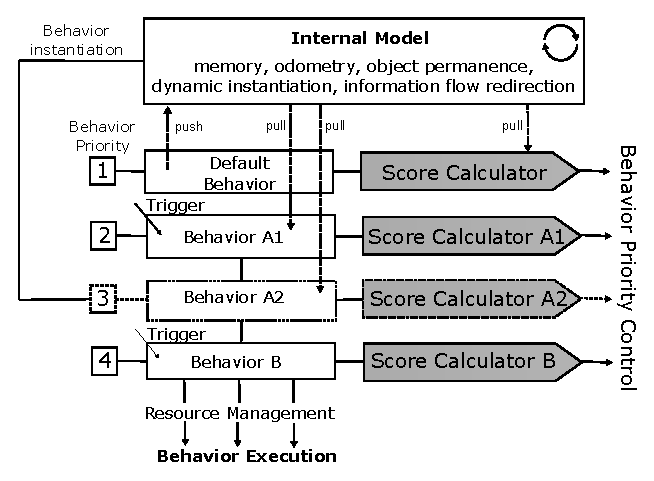
\includegraphics[width=\textwidth]{assets/tdm_im.eps}
%\caption{Information management by IM of TDM}
%\label{fig:tdm_im}
%\end{subfigure}%
%\hfill
%\begin{subfigure}[b]{0.45\textwidth}
%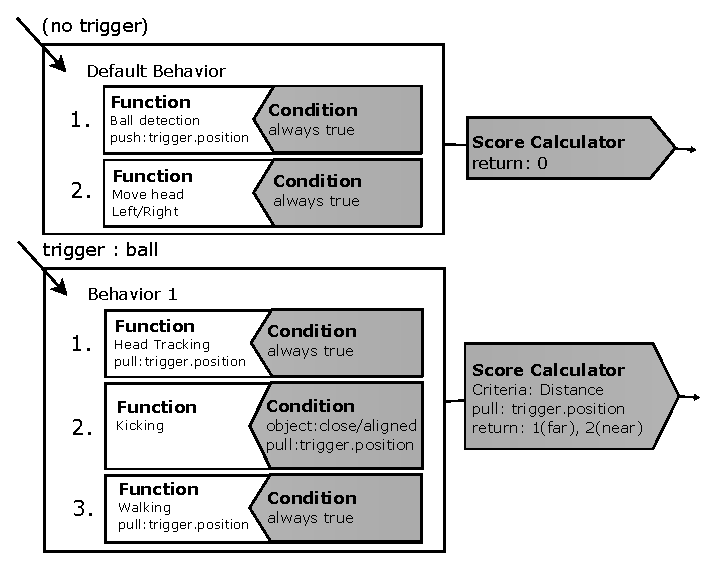
\includegraphics[width=\textwidth]{assets/tdm_example.eps}
%\caption{An example Program in TDM}
%\label{fig:tdm_example}
%\end{subfigure}%
%\caption{TDM Framework \cite{BerenzTDM2014}}
%\label{fig:tdm2}
%\end{figure}
At the time of publication of \cite{BerenzTDM2014}, a visual programming software using TDM was not developed however the user studies were done to understand the usability of such a dynamic behavior programming paradigm. The comparison results of TDM and Aldebaran Choreographe presented in \cite{BerenzTDM2014} indicates that TDM is appropriate when it comes to designing complex dynamic behaviors.
% and results are shown in Figure~\ref{fig:tdm_casestudy}. 
%\begin{figure}[H]
%\centering
%\begin{subfigure}[b]{0.48\textwidth}
%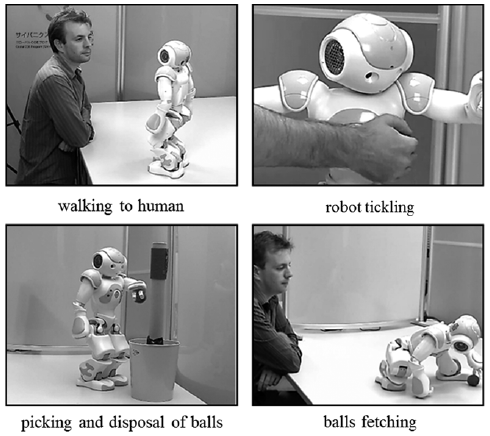
\includegraphics[width=\textwidth]{assets/tdm_casestudy1.png}
%\caption{TDM behaviors used for evaluation}
%\label{fig:tdm_casestudy1}
%\end{subfigure}%
%\hfill
%\begin{subfigure}[b]{0.45\textwidth}
%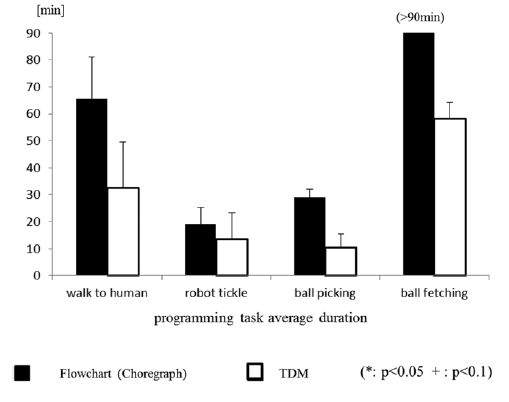
\includegraphics[width=\textwidth]{assets/tdm_casestudy2.png}
%\caption{Programming time for TDM vs Choreographe}
%\label{fig:tdm_casestudy2}
%\end{subfigure}%
%\caption{TDM Usability Study \cite{BerenzTDM2014}}
%\label{fig:tdm_casestudy}
%\end{figure}